\section{Introduzione}
Sempre più giochi da tavolo ormai vantano una versione digitale,
caratterizzata dalla possibilità di permettere agli utenti di giocare in
modalità multiplayer.
Allo stesso tempo però sono ancora rare implementazioni distribuite di
giochi multiplayer le quali spesso sono invece basate su un architettura
client server. In questo documento descriveremo il nostro lavoro di
progettazione ed implementazione della versione software di un gioco da
tavolo con particolare interesse riguardo l'architettura di rete
distribuita utilizzata nella modalità multiplayer.

\subsection{Carcassone}
In particolare è stato nostro interesse occuparci del remake del gioco
da tavolo Carcassonne. Quest'ultimo è un boardgame dei
primi anni 2000 basato su tessere che consiste nel creare un paesaggio medievale 
posizionando e accostando tra loro vari tipi di tessere, che rappresentano una parte di città, 
un tratto di strada, un campo o un monastero \footnote{Si fa riferimento
alla prima versione del gioco in cui non sono presenti fiumi, locande, ponti o altri elementi di paesaggio introdotti dalle varie espansioni}.
Completando più città, strade o monasteri attraverso tali tessere, i
giocatori (previsti da 2 a 5) accumulano i punti necessari a vincere la partita.
Al fine di comprendere al meglio le prossime sezione di questo documento, 
verra` illustrato di seguito il funzionamento del gioco.

All'inizio della partita, una specifica tessera è posizionata sul tavolo, scoperta; 
le altre tessere sono mescolate e rimangono coperte nel mazzo e mischiate.
Ciascuna di tali tessere rappresenta un frammento di paesaggio, e può contenere uno o più dei seguenti elementi:

\begin{itemize}
	\item tratti di strada, inclusi incroci e curve
    \item aree cittadine racchiuse da mura
    \item campi che circondano le città e accolgono le strade
    \item un monastero
\end{itemize}


\begin{figure}[H]
\centering
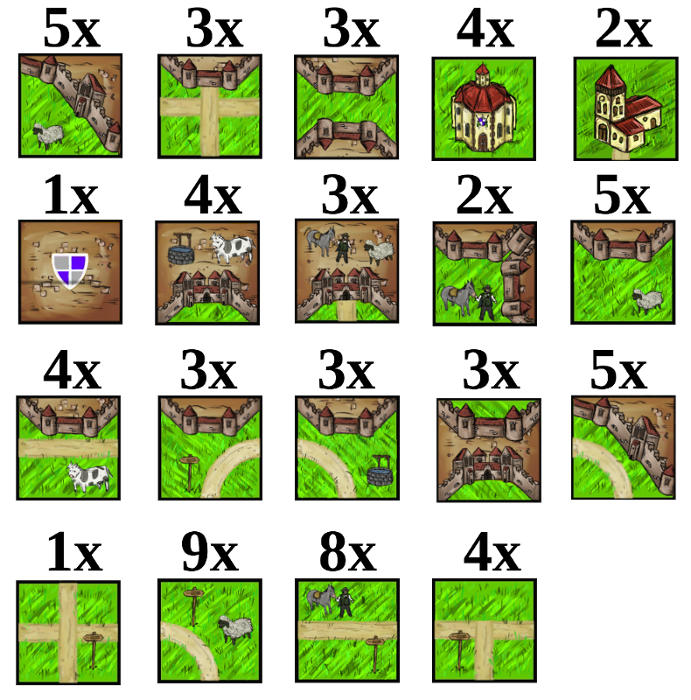
\includegraphics[width=\textwidth]{img/tiles.png}
\caption{Elenco delle tessere presenti nel gioco}
\label{img:tiles}
\end{figure}

A turno, un giocatore per volta estrae una tessera dal mazzo e la posiziona scoperta sul tavolo
a contatto con almeno una tessera già piazzata su uno o più lati, in modo da mantenere la coerenza con le vicine, 
estendendo eventuali strade, campi, o citta` già presenti.

Dopo aver posizionato la tessera, il giocatore può decidere di piazzare
una pedina detta \emph{meeple} su un elemento del paesaggio della tessera appena posizionata, reclamandone la proprietà a patto che non sia già stato reclamato da un altro giocatore.
Può accadere comunque che un elemento abbia più di un
proprietario se diviene una congiunzione di due elementi dello stesso
tipo non precedentemente adiacenti, in questo caso chi ha il numero maggiore di pedine sull'elemento rimane il proprietario, in caso di pareggio entrambi sono ritenuti proprietari e otterranno il punteggio relativo.

Quando un elemento viene completato, se ad esempio le mura di una città
vengono chiuse o se una strada ha due estremità chiuse, il proprietario
di quell'elemento acquisisce i relativi punti e tutte le pedine che erano su quell'elemento vengono restituite ai relativi proprietari. Il punteggio di un
elemento è dipendente dal numero e dal tipo di tessere che lo compongono.

Unica eccezione viene fatta per i poderi, che non vengono mai completati fino al termine della partita e sono soggetti ad un conteggio speciale.

Il gioco termina con il piazzamento dell'ultima tessera, al termine viene effettuato un conteggio finale dei punteggi derivanti dagli elementi non completati ma posseduti dai giocatori che avranno un valore differente in questa fase; vince il giocatore che, dopo il conteggio finale, ha totalizzato più punti.

Rimandiamo alla documentazione ufficiale di Carcassonne per ulteriori
dettagli.

La semplice struttura del gioco e la sua organizzazione a turni rende
interessante l'approccio distribuito in quanto si evita di incorrere in problemi 
di prestazioni tipici dei giochi reattivi. Questi ultimi infatti hanno requisiti prestazionali molto stringenti. In
particolare spesso richiedono che le comunicazioni di rete siano a bassa
latenza al fine di evitare
artefatti grafici fastidiosi dovuti ai ritardi di rete o all'overhead di
comunicazione.\\
Come già accennato, il gioco da noi considerato necessita invece di
requisiti prestazionali più laschi soprattuto per i lunghi tempi
decisionali degli utenti (comparati ai tempi di rete e computazionali).
\\
Vedremo nelle prossime sezioni i dettagli progettuali ed implementativi.
In ultimo forniremo una analisi valutativa dei risultati ottenuti dai test
con le dovute considerazioni finali.
